\chapitre{Timothée craque et remet ça ! le 27 juillet 2033}{L'air de ce petit mercredi de semaine}{ est doux, caressant, aromatisé de tout ce qui, plus au sud, affole les bourdons, les abeilles et les colibris. On voudrait s’y intégrer, s’en faire un linceul, flotter sur son calme courant, se fondre dans la générosité de sa tiédeur veloutée, y rêver sans craindre que le bien-être ne cesse même en se tenant tout près du fleuve en défiant la vigueur des débris salés. On souhaiterait s’encoconner sans retour dans le confort de ce matin de juillet, se perdre dans ces draps de satin blanc, ceux de la nuit incessante, «Nights in white satin, Never reaching the end … », des draps au lyrisme plus prenant que celui de cette froide cotonnade enrobant le vilain trébuchet par où il a fallu passer. Car on aimerait oublier avoir dû sacrifier sa soirée au plus désagréable des stupres, dans la plus angoissante des geôles.  }

On aimerait oublier avoir le cou bien étiré sur une bûche, avoir une meute de chacals déployée tout autour pour la curée, avoir ses proches en grand péril, être en train de naviguer dans un épais cirage sans trop d’instruments fiables. En revanche, on a des amis, peut-être même une amie, sur qui il est possible d’apprendre à compter, si on le veut Pas si mal quand on est un tromboniste involontaire n’ayant pas encore trouvé de passage, aller simple, pour Milet, un binoclard, bedonnant, en chauvaison, recalé socialement. Chauvaison ? Lorsque la calvitie frappe, on tend à se développer un vocabulaire pour en qualifier le processus.

\begin{floatingfigure}[l]{35mm}
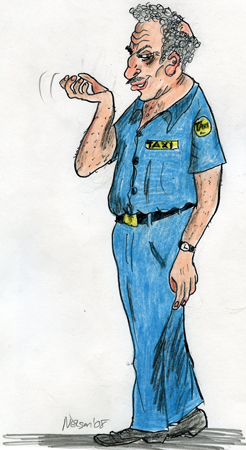
\includegraphics[height=60mm]{corps/chapitre15/img/personnage-jawad.jpg}
\end{floatingfigure}

Entre l’improbable cottage de la rue Crouet et l’immeuble du CRG-BSL, il y a exactement huit feux de circulation. Or, c’est la première fois, depuis qu’il fait ce métier, que Jawad Kebbaj franchi tous ces portails au vert, «Masha’Allah» !

- Il faut prier en initié, mon jeune homme !, dit-il à son rétroviseur à grand renfort de clins d’œil.

Effectivement, à chaque feu, l’ex-médecin marocain psalmodie la formule incantatoire, formule un peu adaptée, mais remontant néanmoins à la nuit des temps, formule qu’auraient utilisée pharaons, dignitaires et nobliaux en quête d’un siège pour que cesse leur errance postmortuaire. Dit-on.

- Laisse-moi passer, feu de circulation, je te connais et je connais ton nom, je connais le nom du dieu qui te garde. Tu t’appelles «Souverain de la peur, aux hautes murailles, le supérieur, souverain de Hebhed, le prophète qui repousse la tempête, qui sauve de la spoliation celui qui vient de loin», ton portier se nomme «le Redoutable» et le dieu qui te garde s’appelle Osiris.

Puis :

- Laisse-moi passer, feu de circulation, je te connais et je connais ton nom, je connais le nom du dieu qui te garde. Tu t’appelles «Souverain du ciel, maître du double pays, l’avaleur, souverain des hommes, contrôleur de tous», ton portier s’appelle «le Rejeton de Ptah» et le dieu qui te garde se nomme Osiris.

Et ainsi de suite, autant de portails-feux, autant de suppliques, autant de permissions divines, autant d’invraisemblances qui contredisaient la conviction de Jawad à l’effet qu’il était mathématiquement impossible de les franchir tous dans la félicité du mouvement continue. Oriris, le dieu aux quatorze morceaux, n’avait-il pas décentralisé la gestion de ses portails, laissant une grande latitude aux portiers, des créatures pas toujours accommodantes envers les humains ? Mais aujourd’hui, tout semblait surréaliste. Par exemple, qui eut cru possible de connaître un matin aussi doux que ceux de Rabat, quand les ardeurs du soleil de juillet sont rafraîchies par la brise de l’Atlantique et les effluves du fleuve Bouregreg ? Mais voilà, tout est concevable en ce bas monde, même la douceur, la joie de vivre et ;e répit. N’en a-t-on pas la preuve en ce début de journée ?

Descendu de la voiture, Timothée remarque une dizaine d’employés, toutes des jeunes femmes, assises, souriantes, heureuses, le nez pointé vers le soleil, comme ces personnages peints sur papyrus dans le Livre des morts. Il s’attarde un instant en ce sérail impromptu, se tourne lui aussi vers la chaleureuse lumière et se laisse caresser. Une préposée toute mignonne lui sourit. Il opine en manifestant un prudent début d’enjouement, mais s’engage néanmoins dans l’édifice. Attention, se di-il, prudence ! Il fait doux, tous les feux ont été au vert et des gens de bonne humeur lui ont témoigné de l’amabilité. Ces invraisemblances sont-elles des indices que sa vie est en voie de se faire belle ? Effectivement, c’est aujourd’hui que Marie-Odile va le débarrasser du docteur Gagnon et qu’elle désamorcera la procédure administrative enclenchée contre lui. Mais à l’inverse, ne serait-ce pas plutôt une façon hypocrite d’indiquer que son existence jusque-là éprouvante est sur le point de devenir cauchemardesque ? Car, après l’intervention de la femme flic, il risque de se retrouver enferré comme jamais, avec, en mains, une facture à payer longue comme la langue de l’homme-tronc.

En route vers les ascenseurs, il est aperçu par Shimoune Saint-Pierre officiant au manger mou qui, ce matin, arbore des nattes blondes lui donnant l’aspect d’une matrone gauloise, une matrone musclée, s’entend. À grands signes, l’énergumène insiste pour que son ami approche. Timothée se faufile alors à travers les vieillards et s’avance jusqu’au comptoir de service.

- Va-t-en vite à la salle du CA. Il est arrivé quelque chose à Dart Vader.

- Quoi ?

- Vas-y vite !

Inquiet, le CS-1 se dépêche dans le couloir encombré pas sa faune matinale et il est dépassé par Tropecolo le Chinois, debout sur sa Saguewanish.

- Qu’est-ce qui est arrivé à monsieur Gagnon, demande-t-il à l’agent de sécurité.

La réponse est tellement dépourvue de tact qu’elle est à la diplomatie ce que l’arrachage soudain d’un diachylon est à la médecine.

- On vient de le trouver mort. Mais t’as le droit d’entrer, c’est ton bénéficiaire, fait-il en rangeant sa trottinette à côté de la porte suprême.

Timothée a une boule dans le gorgoton.

- Il est mort comment ?

- En mangeant. Viens voir.

Dans la salle où flotte une puanteur de diarrhée, Carl Michaud est en pourparler avec Philippe Dauphin, deux employés de la direction générale, à coup sûr des hommes de main du Flipper, regardent la dépouille et Marie-Odile Tremblay parle avec un préposé à l’entretien.

- C’est lui qui a débarré la salle à matin, précise Tropecolo. Méchante surprise !

Dart Vader, la carcasse crispée, les traits révulsés, la bouche ouverte pleine de débris de crevettes, un de ses petits écouteurs décroché de l’oreille, la canule arrachée, du sang coagulé sur le cou, le bas du corps maculé de fécès presque séchées, est étendu par terre, les jambes sous la table, la tête un peu surélevée sur la plinthe en acajou longeant le mur. Autour de lui, de la nourriture gâchée et, sur la table, un désordre de cabarets débarrassés d’une partie de leurs contenus.

Avec son DPP, Tropecolo photographie les deux lettres accolées, celle du CA et celle de Dauphin, tandis que Marie-Odile remercie le pauvre concierge et s’approche de Timothée.

- Tu le connaissais bien ?

- B’en, je l’aimais bien. Il était emmerdant, mais c’était un bon bonhomme.

- Tu penses à quoi quand tu vois le corps amanché de même ?

- Ça me semble clair qu’il a étouffé. Mais je comprends pas le sang.

- Moi c’est les deux portes barrées de l’extérieur, celle de Dauphin et celle du CA, que je comprends pas.

L’agente pointe don index vers l’oreille gauche de cadavre où l’écouteur est toujours en place.

- As-tu une idée de ce qu’il écoutait ?

- Il aimait bien écouter de la musique québécoise, de la chansonnette française. Il connaissait Mouloudji par cœur.

- Qui ?

- Mouloudji.

- Mou … De toute façon, ça va être analysé.

Leur attention se porte alors sur le directeur des communications qui a commencé à crier dans sa boucle d’oreille.

- Allô ! Oui c’est moi, qui c’est qu’tu veux qu’ce soit d’autre ? Envoi, shoot ! Le point de vue officiel ? Le bonhomme est mort d’une indigestion. Une mort royale ! C’est ça ! Essaie de trouver le moyen de comparer avec la mort du roi Adolphe Frédéric de Suède. Oui. Adolphe Frédéric de Suède. Ça s’est passé en 1771. Il est mort après avoir bâfré en une seule ripaille des quantités abominables de homards, de caviar, de choucroute, de coleslaw, de kippers et de poisson fumé, sans oublier quatorze portions de semla. Hein ? De la semla c’est une sorte de chou à la crème servi dans un bol de lait chaud, ouin, du lait chaud, le tout b’en arrosé de champagne. C’est ça. Le bonhomme aura commis une dernière extravagance. Le CA ? J’ai des gens qui communiquent présentement avec les membres pour leur dire que la réunion est remise sine die. OK. Bye.

Carl Michaud qui a lui aussi été obligé d’écouter le monologue du Flipper, s’en approche vivement.

- Avec qui parlais-tu ?

- Avec Angélique, ma responsable des relations médias.

- Écoute-moi bien, Philippe. On n’admet rien. On ne dit rien. Le vieux chnoque est mort de sa belle mort.

- Il a prévenu les médias et Dennis-Dubeau de ses intentions; ils vont rappliquer, ils vont nous écœurer.

- Tu leur diras qu’il ne s’est rien passé.

- OK boss !

- On fait venir les gars du frigo, on le met le bonhomme dans un sac zippé et on le grille à la prochaine cérémonie.

En entendant la décision du directeur général, Timothée ressent une montée d’adrénaline.

- Excusez-moi, monsieur, mais on n’a pas le droit de faire ça.

Carl Michaud lui jette un regard chargé d’embûches létales, de trappes fatales, de lames empoisonnées, de grosses misères et de mille dangers. Mais il n’a pas le temps de répliquer. Tropecolo s’est avancé.

- Tardif a raison, monsieur. Nous sommes en présence d’une mort suspecte. Il y a du sang, du bordel, la victime n’avait pas d’affaire ici, elle était enfermée sous clé, son visage est convulsé, ses membres crispés et sa bouche pleine de nourriture. Et il venait de passer quasiment une semaine en prison sans aucune justification administrative. C’est louche. Pour le moins. Dans un cas comme celui-là, la loi nous oblige à en référer à la police, qui, à coup sûr, va faire venir un médecin légiste.

- B’en voyons ! On va quand même pas déranger les flics pour une niaiserie de même, s’objecte Philippe Dauphin.

- J’ai bien peur que oui, mon Flipper.

- De toute façon, coupe Marie-Odile, il est trop tard pour s’astiner, je viens de les appeler. Ils vont être ici dans quinze minutes.

Visage convulsé, membres crispés, bouche pleine de crevettes, excréments, Timothée est intrigué. Et si c’était une réaction allergique ? Le vieillard souffrait peut-être d’intolérance par rapport à certains aliments. Apercevant le terminal quantique sur une table au fond de la salle, il ouvre une session et se fait sortir le dossier Robert Gagnon, 5e Nord. Or rien n’apparaît au rayon allergies. Rien !

Au même moment, il entend la voix de Marie-Odile.

- Chinois, va voir vite !

Elle pointe en direction du bureau de Dauphin. Tropecolo y découvre le haut gradé en train de gratter la feuille que Dart Vader avait accolée en début d’orgie à sa table de travail.

- Flipper, arrête. Tu n’as pas le droit. Ne touche plus à rien, ordonne-t-il.

- Tout le monde doit immédiatement sortir, corrobore Marie-Odile. Seuls Tropecolo et moi pouvons rester en attendant la police.

Comme Dauphin ne semble pas faire de cas de l’avertissement, Tropecolo revient à la charge.

- Monsieur, ce que je dis et vois présentement est numérisé par mon DPP. La feuille que vous essayez d’arracher a été filmée plus tôt et ce que vous êtes en train de faire est illégal et pourra être retenu contre vous.

- ‘Stie de zélé, lui rétorque le cadre administratif qui déguerpit.

Apercevant Timothée en train de refermer le terminal, il poursuit sur le ton «mesure de guerre».

- Vous aussi, monsieur Tardif, je vous ai dans mon DPP. Vous devez quitter cette pièce immédiatement.

Le CS-1 le regarde avec une certaine douceur.

- Merci Tropecolo, merci Marie-Odile. J’apprécie votre rigueur. Monsieur Gagnon le mérite.

Dans le couloir, il se gratte le crâne et, sans hésiter, il descend au sous-sol et fonce en direction sud vers le laboratoire du docteur Bellavance. La salle d’accueil est plutôt exiguë, mais la jeune femme qui y est affectée est agréable à zieuter avec son petit nez retroussé. Elle paraît encore sous le charme du soleil matinal devant lequel elle a dû s’attarder tout à l’heure.

- Tu peux entrer, lui dit-elle en pointant vers une porte à sa gauche. Il t’attend dans son bureau. Ça va être complètement au fond, à ta droite.

Timothée doit alors traverser une grande pièce comptant une vingtaine de lits où semblent dormir des zombis intubés, des morts maintenus vivants et socialement utiles, d’anciens ingénieurs, fonctionnaires, commerçants, pêcheurs, enseignants, avocats, menuisiers, hommes et femmes, devenus des matrices à hormones, des animaux inertes que l’on entretient et que l’on trait ou tond. Si la plupart sont seuls, certains ont l’insigne honneur d’avoir une porteuse de sarrau, quelque instrument en main, en train de leur contrôler le truc du machin de la patente, de leur gratter un bout de peau, de leur tapoter un tube ou de leur vérifier un signe vital. Ne sachant plus comment ne pas regarder cette scène d’horreur, le CS-1 aboutit dans le grand bureau du médecin chercheur où il est accueilli avec chaleur.

Il a tôt fait de lui raconter dans le détail ce qu’il vient de voir dans la salle du CA et lui fait part de son questionnement sur la possibilité d’une violente réaction allergique.

- Avez-vous des connaissances médicales, monsieur Tardif ?

- Un peu, j’ai quasiment un DEC en soins infirmiers.

- Je comprends vos interrogations et la justesse de la piste que vous envisagez d’approfondir.

- Euh …

- Vous avez sûrement entendu parler de choc anaphylactique ?

Et le médecin de lui rappeler la nature éminemment dangereuse de cette pathologie, une réaction allergique exacerbée pouvant entraîner la mort. Si personne n’est sur place pour lui administrer de l’adrénaline, le patient a alors de très bonnes chances de trépasser. On parle d’une chute précipitée de la pression artérielle, de tachycardie, de troubles respiratoires, de vomissements et de diarrhées, le tout dans les minutes qui suivent l’absorption de la substance irritante.

- Ça ressemble à ce que je viens de voir, sans les vomissements.

- Attention, ce n’est qu’une piste que le médecin légiste devra explorer.

- Mais docteur, la fiche patient de monsieur Gagnon n’indique aucune allergie.

- Dans l’hypothèse d’un choc anaphylactique, ça veut dire qu’entre le moment où elle a été complétée, la fiche, et le moment de sa mort, au monsieur, il peut très bien en avoir développé une allergie, pour peu que cette piste soit la bonne. Et ici, j’aurais envie d’accuser les crevettes, une nourriture fortement iodée qui n’en est pas à ses premiers méfaits.

- Mais pourquoi il aurait saigné ?

- Faudra voir avec le médecin légiste.

- Depuis trois ans qu’il est ici, monsieur Gagnon n’a été nourri qu’au Nutrisuz. Pourrait-il y avoir un lien de cause à effet entre cela et le développement d’une allergie ?

- L’hypothèse est intéressante et mériterait d’être vérifiée.

Le docteur Bellavance plonge ses yeux invasifs dans ceux de Timothée.

- Monsieur Tardif, on peut parler librement. J’ai obtenu qu’ici au labo, rien, ni conversation, ni action, ne puisse être enregistré à la Sécu.

S’il y a lien, explique-t-il, si la piste tient la route, les protagonistes du Nutrisuz risquent d’avoir l’air un peu fou; ils pourront avoir des comptes à rendre. Pour le moins, il y aura enquête à la grandeur du Québec, peut-être même du Canada, si le Fédéral s’en mêle. Depuis qu’on administre cette rinçure chimique aux vieux, combien sont décédés à la suite d’un choc anaphylactique ? Sera-t-il possible de vraiment le savoir avec cette manie qu’ont les CRG de tout gommer, de tout mettre en sac, de tout faire disparaître à chaque mois lors des cérémonies ? Rien ne sera moins limpide. Il faudrait partir à zéro, procéder par échantillonnage de bénéficiaires que l’on remet à la vraie nourriture, les suivre repas par repas. Et, pour arriver à une telle étude, il serait essentiel qu’au départ il y ait des pistes significatives. Pas seulement au Québec. Peut-être même aux États-Unis ou ailleurs au monde où de telles politiques gériatriques ont été implantées.

- Ce que je vous dis, monsieur Tardif, c’est que tous les Michaud et Dauphin du réseau, tous ces profiteurs, vont faire tout en leur pouvoir pour étouffer cette histoire. N’est-ce pas là qu’une affaire banale de personnes âgées qui passent l’arme à gauche ? Crever d’allergie ou du cancer ou d’un infarctus ou d’une surexposition aux ondes, ce n’est que mourir. Tout le monde connaît son heure. Pourquoi devrait-on s’exciter les lobes d’oreille là-dessus ? Pourquoi est-ce que ça devrait devenir un scandale médiatisé ? Si la société vote massivement pour des politiciens qui encagent les vieux et les nourrissent au Nutrisuz, pourquoi trouverait-elle répréhensible que certains décèdent à la suite d’un choc anaphylactique ?

Pénétrer dans l’antre du diable, dans la grotte cachée d’un savant fou, dans la cave sinistre du docteur Frankenstein, pour se faire asséner une telle vérité relève du prodige.

- Et je les connais bien ces profiteurs, continue le toubib. Je pourrais vous en parler, monsieur Tardif.

- Euh …

- Je pourrais même vous parler de trafic d’hormones.

- Euh … Attendez, attendez, docteur, pourquoi vous me dites ça à moi ? Croyez-moi, j’ai plus vraiment de place dans ma pauvre tête.

- Pourquoi ? Simplement parce que vous êtes honnêtes et que, bien malgré vous, vous avez présentement à les combattre, ces Michaud et Dauphin. Et je dispose de certaines preuves irréfutables que mon travail ici n’enrichit pas le Centre tel que prévu au départ du projet, mais la poche d’une petite mafia dont Michaud et Dauphin sont deux représentants, une mafia régionale dont fait partie Pete Barrett, l’homme des basses œuvres de Sylvain Turcotte, notre bien-aimé député ministre. Connaissez-vous Claude Sey ?

- Oui.

- Il est en danger et il le sait. Nous avons travaillé de concert sur la découverte du pot aux roses.

Timothée a atteint son seuil de tolérance. Le crâne lui travaille fort pour éclater.

- Docteur, on s’en reparle. Je dois filer. Je suis très en retard.

- Quand vous voudrez, monsieur Tardif, mais ne tardez pas, j’achève, ici.

- Vous partez ?

- Disons qu’on ne me fait plus confiance.

La première personne sur qui le chef de section tombe lorsqu’il arrive au 5e Nord, c’est Jean Saint-Gelais. Il s’avoue consterné et prévient qu’il va venger Dart Vader. Il ne sait pas comment, mais il est certain qu’il le fera. Timothée est encore en train d’essayer de se débarrasser du bonhomme quand Ronnie Ross lui fait signe de venir le joindre derrière le comptoir du poste de garde. Il a la mine plus basse que normale.

- J’sais pas comment t’annoncer ça, Motté, mais faut que j’te dise que les deux Martel, tes amis de la petite chambre, Laurent p’is moi, on vient de les retrouver morts tous les deux.

Le coup est violent. Imparable.

- Morts ? Comment est-ce possible, câlisse !

- On a rien touché, viens voir.

L’un à pied, les deux autres en Saguewanish, le trio arrive devant la pièce en question où Ronnie dicte le code d’ouverture. Dans le petit lit, l’homme et la femme reposent côte à côte, les traits paisibles, on jurerait deux vieux amants faisant la sieste. Par terre, une feuille de papier sur laquelle on a écrit :

    Comme en 2033, la vie des vieillards n’a d’autre sens que celui de ce rapprochement quotidien d’un grabat dans la salle palliative en attente de la Cérémonie mensuelle, nous pensons que ce n’est plus notre place ici et qu’il est préférable aller voir ailleurs si c’est mieux. Grand merci à ceux qui, comme le Chef du 5e Nord, ont essayé d’améliorer notre sort. Quant aux autres, qu’ils se disent que nous avons fini de les haïr.

Il n’y a pas l’ombre d’un doute; c’est encore une histoire de pilule du bonheur. Les yeux mouillés de larmes, Timothée arrive à peine à répondre aux deux préposés qui veulent savoir comment procéder avec ce double décès.

- On fait comme d’habitude. La routine câlisse. On fait comme si on ignorait qu’ils se sont suicidés et on appelle les gars du frigo. Ensuite, vous connaissez la marche à suivre. Et moi aussi. Deux de partis, deux d’arrivés. Deux dossiers à fermer, deux nouveaux à ouvrir. Encore des câlisses de statistiques à modifier.

- OK Motté.

La journée avait pourtant si bien commencé se dit le CS-1 en longeant le mur en direction du bureau de Robespierre Alcide.

Quand elle le voit entrer et s’écraser sur la chaise libre, Mme Bellow juge à propos de sortir prendre sa pause promenade.

- Ou-là-là, fait le colosse.

- Ils sont morts tous les deux, Robespierre

- Qui ça ?

- Viens pas me dire que tu le sais pas ! C’est pas toi qui les distribues, les câlisses de pilules ?

Le gaillard ne bronche pas.

- À matin, Robert Gagnon, maintenant, les deux Martel, maudit que la vie est moche !

Et tel l’enfant qu’il avait probablement cessé d’être à l’époque du Lac Saint-Mathieu, Timothée éclate en sanglots. Un sanglot profond, puissant, ancien, total, siphonnant. Un sanglot chargé de douleur que tout le 5e Nord doit entendre en baissant la tête. Un sanglot d’un désespoir tel que personne ne l’oubliera jamais. Incapable de se retenir, Robespierre s’approche de la chaise, se met un genou à terre, relève délicatement la tête de son ami et se la place sur l’épaule. Puis, de ses grands bras, il lui enserre doucement le haut du dos et se met à lui répéter, telle une comptine :

- Laisse-toi aller mon ami, laisse tout le mauvais sortir.

À l’arrivée des policiers dans la salle du CA, Marie-Odile avait jugé que sa présence n’était plus essentielle. Par contre, son collègue Tropecolo étant celui qui avait tout capté avec son DPP, ne demandait pas mieux que de rester sur place avec les flics de la grande maison ce qui, dans sa tête, lui conférait beaucoup d’importance, sans parler de l’expérience. Peut-être même pourrait-il développer un contact et avoir sa chance d’être admis dans la ligue des vrais.

Après s’être assurée de la disponibilité de Béatrice Martin, elle s’était mise en route vers la demeure de l’infirmière en congé maladie et sur le point d’être en recherche d’emploi. Car pour elle, il n’était plus question de retourner en Haïti; sa santé lui rendant désormais ce scénario impensable.

- Bonjour, dit-elle à Marie-Odile en ouvrant, je suis Béatrice Martin.

L’apercevant toute souriante dans le cadre de porte, la femme flic comprend qu’il va lui falloir trimer dur pour ne pas perdre Timothée. Non seulement cette femme est beaucoup plus jolie qu’elle, mais son sourire est la merveille des sept mers, son aura une féerie vibrante sur laquelle on veut se réchauffer, sa peau, en tout cas, celle de sa main qu’elle serre, d’une douceur à se faire lesbienne ad perpet. Et ces yeux qui brillent comme ceux d’une Sainte-Vierge éclairée aux lampions. Et cette petite robe qu’elle peut porter, elle, et qui la fait paraître comme incarnant la quintessence de la féminité, un look qui rend les hommes dingues et qu’elle, la grosse Tremblay, n’a jamais pu se permettre de sa chienne de vie. Marie-Odile évalue qu’à âge et taille sensiblement égales, la pimbêche doit traîner une vingtaine de kilos en moins qu’elle, une «tomboy» plus barattée qu’ondulée. Du coup, elle la déteste d’une haine sourde comme celles qui tétanisent les muscles maxillaires jusque dans l’inconfort, comme celles qui fait en sorte qu’on regarde calmement, en souriant, quelqu’un se noyer en se fichant de se faire accuser de non-assistance de personne en danger de mort, comme celles qui ont inspiré des générations de fabricants de poupées vaudou.

Sauf que l’agente de sécurité est une professionnelle. Elle sera froide et distante, mais elle demeurera polie et respectueuse. Rien de sa rancœur ne paraîtra. Elle captera sa déposition selon les règles de l’art, se la fera jouer pour vérification, remerciera la belle infirmière et, de sa démarche lourde, masculine, s’en retournera à sa voiture de fonction.

C’est le pauvre docteur Gagnon, un autre dont Marie-Odile s’était assuré de la présence, qui subira les conséquences de ses vingt kilos en trop de et de sa dégaine de perdante dans un contexte où la gagnante est une déesse.

À la manière d’un livreur d’eau en bouteille, elle pénètre dans la clinique et, de la façon la plus naturelle du monde, demande où se trouve le bureau du bon docteur. La réceptionniste pointe vers une porte, mais se dépêche d’ajouter que son patron est en consultation. Cela ne décourage pas l’intruse qui continue vers le local indiqué, cogne et entre sans attendre d’invitation. Une patiente, le genre friqué dont les fringues doivent coûter trois fois le salaire mensuel qu’on verse aux agents classe 1 au CRG-BSL, la regarde sans broncher. La pièce embaume le parfum horriblement cher.

- Qu’est-ce qui se passe ? demande Étienne Gagnon.

- Y’s passe que madame, ici là, s’en va patienter deux minutes dans la salle d’attente. Ce que j’ai à vous révéler, monsieur, ne la concerne pas du tout.
Le praticien hausse le ton.

- Vous êtes qui, vous ?

Affichant l’air le moins séduisant du monde, Marie-Odile Tremblay présente sa plaque d’agente de sécurité au CRG.

- Je vous répète, monsieur, que ma visite ne regarde que vous, personnellement.

- Allez m’attendre à l’accueil, je serai à vous dans vingt minutes, lui dit-il avec morgue.

- Ah bon ! C’est comme ça que vous voulez la jouer, la partie. Parfait. Je vais vous parler devant la madame. J’enquête, monsieur, sur un complot visant à voler des produits pharmaceutiques au Centre à la suite de traitements que vous avez consentis à une dame âgée du quartier Nazareth, plus particulièrement sur la rue Crouet, une certaine Marie ….

- Ça va, ça va ! Madame Robert, vous voulez me donner quelques instants ? Je suis à vous dans deux minutes.

Sans parler, la patiente ondule sur ses escarpins presque échassiers vers la porte et disparaît entraînant avec elle une fragrance susceptible de transformer n’importe bière en jus de chaussette. Marie-Odile referme l’huis et se tapote la boucle d’oreille.

- Je suis ici pour prendre votre déposition dans une affaire impliquant le chef de section Timothée Tardif. J’ai ici, dans ce petit dispositif, deux témoignages officiels dont copies sont déjà dans le serveur de la Sécu au Centre. Il y a celle de monsieur Tardif qui prétend être venu vous chercher d’urgence, le mercredi 20 juillet dernier, pour vous amener traiter une de ses amies, madame Béatrice Martin, une infirmière en congé maladie, pour des raisons médicales qui n’intéressent pas mon enquête. Cette déclaration est corroborée par celle de Mme Martin qui reconnaît que vous lui avez procuré à ce moment et à trois occasions par la suite, des soins de grande qualité.

- Qu’est-ce c’est que cette histoire farfelue ?

- J’y arrive. Vous allez maintenant me déclarer la même chose. J’en ferai votre déposition officielle et j’irai clore mon enquête.

Gagnon est abasourdi.

- Vous êtes folles, dit-il en direction de son terminal. J’appelle Carl Michaud immédiatement.

Elle lui jette un disque mini 3DVD.

- Je ne ferais pas cela à votre place. Voici votre dernière conversation avec monsieur Tardif. Si vous vous donnez la peine de visionner cette copie certifiée et numérotée par la Sécu, vous constaterez que vous lui consentez un délai pour qu’il vous vole des produits pharmaceutiques. Je refile ça à n’importe quel flic et vous être arrêté. Je refile ça à n’importe quel journaliste et votre réputation est détruite.

Si les yeux humains disposaient de fonctions lance-flamme, Marie-Odile Tremblay ne serait plus qu’un amas de suif en train de fondre.

- En résumé, nous allons nous entendre sur trois choses. Un, vous me faites une déposition dans le sens que je vous ai suggéré tantôt. Deux, vous oubliez définitivement monsieur Tardif pour vous procurer des produits pharmaceutiques. Trois, vous éliminez de votre mémoire tout ce qui est relatif à ses parents. Si vous dérogez à ces trois conditions, je vous détruis.

- Est-ce qu’ils sont tous aussi baveux que vous, à la Sécurité du Centre ?

- Votre réponse, monsieur ?

- Je me plie à votre chantage, mais vous pouvez être assurée, madame la «grosse police», que la mère de votre ami Tardif, elle pourra crever avant que je remette les pieds là.

- C’est un beau geste de votre part, monsieur. Les malades craignent les rats; ça leur donne des cauchemars.

Vingt minutes plus tard, Marie-Odile est de retour au CRG avec, dans sa besace, deux dépositions hautement favorables à Timothée dont l’une contient l’expression indélébile d’une haine éternelle. Elle a tôt fait d’en tirer un rapport qu’elle dicte à son système et qu’elle téléverse dans la boîte d’accueil de la direction générale. Les grandes lignes ? Le CS-1 Timothée Tardif est blanc comme neige. Rien d’illégal ou de contraire aux intérêts du CRG-BSL ne peut être retenu contre lui. Idem pour le docteur Étienne Gagnon, médecin visiteur audit CRG-BSL.

Le mieux, se dit-elle en ravalant son cafard, serait maintenant de monter au 5e en avertir l’intéressé lui-même. Son excellence l’intéressé, sa sérénissime splendeur, sa très haute grandeur toute potelée, Sa Majesté toute pansue qui, effoiré au sommet de ses trois cent trois coussins moelleux, lui condescendra, à elle, cette femelle parmi tant d’autres femelles, à la condition qu’elle le mérite, cela va de soi, un regard, peut-être même un geste pouvant être interprété comme quoi il la juge sur la bonne voie, celle menant au plaisir inouï, unique, recherché, de se faire honorer par sa virilité prodigieuse de grand homme, schlac, ouf, ouf, iièèii, euh ! Elle rumine, la Marie-Odile, elle broie du noir, elle transpire du vinaigre, elle digère ses sucs gastriques, elle grince des dents, elle se hérisse le poil des aisselles, elle s’escrime les hémorroïdes, elle téléporte des ondes létales à cette Béatrice Martin, rombière, princesse, gédaille, nouvelle maigre qui doit avoir le ventre, les seins et le cul striés de vergetures, sans parler du haut des cuisses qui doit être picoté de cellulite, cette ancienne jeune aux petits sourires hypocrites, traîtres, qui n’attend qu’un cave avec du fric pour en être la sangsue. Un cave comme Timothée, imbécile aussi déluré qu’un poisson rouge, qui rampera pour lui lécher le dessous des semelles. Oui mais Timothée n’en a pas de fric. Quel salaud quand même ! Tous des salauds ! Après ce qu’elle a fait pour lui, au risque de se faire attraper et de perdre son boulot. Les hommes ! Tu leur consens un pouce, ils prennent un pied.

Comme elle s’apprête à monter lui déverser quelques litres de fiel, des crampes lui rappellent ces quelques années à tirer avant de frapper sa ménopause. D’où sa déprime et sa jalousie, qu’elle conclut. N’empêche que le fils Tardif et un beau salaud et cette Martin, une belle gourgandine, une marie-couche-toi-là de la pire espèce, celle des petites kioutes à qui tu donnerais le Bon Dieu sans confession.

De si agréable humeur, elle saute sur sa saguigi et file en direction du 5e Nord. Parce qu’au CRG-BSL il n’y a ni poules en liberté, ni marmotte qui traversent les couloirs, ni enfants en train de jouer, elle n’en écrase aucun. Elle sort de l’ascenseur tellement vite, qu’elle évite de justesse de frapper Robespierre.

- Tout doux, Marie-Odile. Y a assez eu de morts pour la journée.

- Excuse ! Ça va assez mal de même !

Comme elle semble se diriger vers le bureau de Timothée, il la hèle.

- Excuse-moi, tu t’en vas chez notre ami ?

Elle ralentit et hoche affirmativement de la tête.

- C’est pas de mes affaires, mais si tes états d’âme le concernent, si t’es pour lui dire des choses désagréables comme il les mérite sûrement, t’es quand même une femme de qualité, il faudrait peut-être que tu m’écoutes un instant.

Puis, se tournant vers Mme Thériault qui fait mine de ne rien entendre, il sourit.

- Bonjour madame, je peux vous aider ?

La vieillarde ne répond pas et disparaît en direction du salon communautaire.

- Envoille, je t’écoute !

- Voilà. Timothée en a plein le casque : Dart Vader en arrivant, deux de ses bénéficiaires qu’il appréciait particulièrement un peu plus tard. Je l’ai ramassé à la petite cuillère tout à l’heure; t’as pas idée ! Crois-moi, il n’est plus capable d’en prendre. Si tu lui dis des choses méchantes, c’est certain qu’Il va tilter. Je l’ai jamais vu aussi abattu. Sérieusement, ce n’est vraiment pas le moment d’en rajouter.

Il lui a mis ses grosses paluches sur les épaules.

- T’as pas le choix, ma grande. Ravale ta colère et donne-lui un break. Garde ça pour un autre jour.

Elle semble hésiter.

- S’il te plaît ?

- Bon, OK !

Lentement, il retire ses mains et la gracie du plus Alcide de ses sourires.

- Si je peux t’aider, fais-moi signe.

Et le Robespierre de s’effacer.

Timothée est assis à son bureau en train de consulter un album de photos d’environ dix centimètres d’épais, le type cartable vendu en pharmacie. Photos noir et blanc des années 1930, 40 et 50, photos couleur, souvent délavées, à partir des années 60, photos numériques découpées, le bleu presque disparu, dès l’An 2000, belle jeunesse sur des skis de bois durant l’hiver 1943, scènes de la conflagration rimouskoise de 1950, gamins quasiment en joie devant des mononks endimanchés, petite bière en main, paquet d’enfants hilares dans un Mercury Meteor 1962, photos de diplômés les cheveux plein de colle, couple souriant sur un sofa orange et brun contre un mur décoré pour Noël, jeunots surex à l’Expo 67, alignement de quelques aînés avec, au centre, deux jeunes mariés, fêtes, anniversaires, voyages, plage, neige, camping, mer, personnages d’âge certain, d’âge très certain.

- C’est tout ce qui reste de leur vie, dit-il à Marie-Odile sans la regarder. Des photos banales, plates. Des clichés de leur routine annuelle. On les voit ensemble pendant une bonne soixantaine d’années. Elle semblait belle et lui, il avait l’air fier. On dirait qu’ils n’ont pas eu d’enfants.

La femme-flic fait un lien avec les «deux bénéficiaires» décédés et laisse le monologue durer encore quelques instants.

- J’suis désolée, soupire-t-elle. Mais j’viens pas pour ça. C’est pour te confirmer que j’ai terminé mon rapport et que je l’ai uploadé dans la quiou de la direction générale. Fait que t’es blanchi, témoignages à l’appui. Pour l’instant, ils vont devoir te sacrer patience. Je dis bien «pour l’instant». Du côté de Gagnon, il a perdu ses dents. Lui non plus, il peut plus t’embêter. Pour l’instant. C’est au moins ça comme bonnes nouvelles, non ? Mais il y en a une mauvaise.

Timothée la regarde comme une victime d’indigestion qui lorgnerait un immense plat de choucroute.

- La mauvaise, continue-t-elle, c’est que cet enfant de chienne a décidé de ne plus jamais mettre les pieds chez ta mère. Si on le force pas, va falloir trouver quelqu’un d’autre. Et si on le force, ça risque d’être aussi pire. Imagine ta mère.

Il retire ses verres et les glisse entre deux boutons de sa chemise pour les essuyer.

- B’en y a Béatrice Martin. Elle est infirmière et hier, elle a m’a dit qu’elle pourrait peut-être passer. Je vais lui demander.

Incapable de se contenir, Marie-Odile se lève brusquement, tous les muscles du visage traités aux hormones de croissance. Heureusement, la mine de Robespierre lui revient et arrive à calmer ses volcans internes. Elle se contente de dire qu’elle ne se sent pas bien, qu’elle a ses menstruations difficiles, qu’elle doit aller prendre des médicaments, qu’elle va probablement rentrer chez elle pour se coucher, bref, que leur tête-à-tête de soirée est remis à un autre jour. Puis, avant même qu’il n’ait le temps d’accuser réception à cette ouverture de cage, une ouverture contre toute attente, elle attrape sa trottinette et disparaît.

Exit Ilsa la louve ! Non sans soulagement, il se replonge dans l’album des Martel. Mais sa tête est ailleurs.

- Béatrice Martin, dit-il à son terminal.

Le système se retrouve bredouille.

- Il ne semble pas y avoir de fiche correspondante, serine la machine.

- Information, Rimouski, rue Pouliot, Martin B.

- Il y a une seule inscription répondant à ces critères. Voulez-vous que je l’ajoute à la liste des contacts ?

- Oui !

- Coordonnées ajoutées. Voulez-vous que j’appelle ce nouveau contact ?

- Oui !

Les aveugles qui ont à se constituer l’image mentale d’un interlocuteur adoreraient sûrement parler à Béatrice; ils en tomberaient amoureux à coup sûr. Autant cette femme est belle, chaleureuse, agréable et séduisante, se dit Timothée, autant sa voix est chaude, empathique, vivante et sensuelle. On jurerait que tous les anges du ciel font le cercle autour d’elle pour que chacune de ses paroles soit un vrai moment de bonheur. Au téléphone !

- C’est Timothée Tardif, euh, du CRG…

L’idiot ! Pourquoi lui a-t-il fallu préciser l’origine de son salaire. Comme s’il trouvait normal qu’elle ne le replace pas, qu’il se pouvait qu’elle ait déjà oublié le fils Tardif à qui elle avait remis une si terrible lettre, comme s’il voulait garder ses distances en se cachant derrière son foutu centre gériatrique. Tant qu’à y être, pourquoi ne recommencerait-il pas le vouvoiement !

- Moi c’est Béatrice Martin, bachelière en nursage provisoirement en convalescence, monsieur du CRG, qu’elle répond avec, on peut imaginer, un petit sourire moqueur. Je le sais bien que c’est toi !

- Euh, ouais. Euh, je voulais te parler du docteur Gagnon.

Et il lui relate l’essentiel de la visite de Marie-Odile. En un mot, le médecin profiteur a été neutralisé, l’enquête interne renvoie Michaud et Dauphin à la case de départ, la pression est devenue un peu moindre, mais il n’y a plus personne pour offrir de soins à sa mère.

- B’en voyons Timothée, je suis là !

- Mais ça n’a pas de bons sens de t’embarquer dans une histoire de fous comme ça.

- Pourquoi ?

- C’est rien de bien drôle, ma mère est un peu spéciale. P’is t’es en convalescence et, j’sais pas moi, s’il surgissait quelque chose de grave ? Tu serais mal prise.

- Tu veux dire «grave» comme seul un docteur peut traiter ?

- Ouin. P’is en plus, je sais pas trop comment on va faire pour payer tes honoraires.

- Mes honoraires ? Quels honoraires ? Est-ce que tu penses vraiment que je suis une personne qui essaierait faire des sous avec du bon monde comme vous autres ? Écoute, espèce de fils inquiet cassé comme un clou, en quinze ans de dispensaire bénévole en Haïti, j’en ai vu de toutes les couleurs et je pourrais en montrer à plusieurs médecins, surtout aux jeunes fiers-pets qui croient tout savoir. P’is de l’argent, j’hais ça !

Timothée s’en veut tellement qu’il se frapperait la tête contre ses murs en béton. Quel con, mais quel con, il est ! Il a la chance de parler à la plus belle femme de la planète, lui dont l’exercice récent du romantisme a pour cadre un stalag, il a le privilège de tenir au bout de la ligne la personne la plus chaleureuse, la plus douce, jamais croisée dans sa mocheté d’existence, il réussit à lui faire hausser le ton, il ne fait qu’accumuler les impairs. Pendant une minute ou deux, il va ainsi essayer de remonter la pente. Maladroitement. Il va prétexter sa confusion mentale, sa fatigue et l’état de sa journée qui n’est pourtant qu’à moitié passée.

Et elle, la bonne Rapuntzel, elle va l’aider. Elle va lui affirmer comprendre sa situation, «j’ignore comment tu fais pour survivre à autant d’ennuis». Elle va lui ouvrir toutes grandes ses portes. Elle va lui raconter qu’au dispensaire, ils avaient recruté un médecin, un Québécois qui désirait s’impliquer pour soulager la misère des Haïtiens. Mais à peine débarqué, il avait voulu prendre le contrôle des opérations et s’était mis à traiter Béatrice comme une assistante sans envergure, «quand on est payé des pinottes, n’est-ce pas ?» Pire, pendant des mois, il avait tenté de s’en faire une maîtresse. Excédée, elle lui avait rivé son clou en faisant ressortir son insuffisance professionnelle. Le gars posait parfois de mauvais diagnostics et il lui arrivait de se tromper dans ses prescriptions. Voyant en elle une coopérante apparemment plus compétente, assurément plus fiable et manifestement plus appréciée des gens, les autorités de la clinique avaient renvoyé chez lui le prétentieux toubib.

- Le problème, c’est qu’on n’a jamais pu le remplacer.

- Mais pourquoi t’as pas choisi de te faire médecin au lien d’infirmière ?

Quel con, quel con, mais quel con !

- Parce que mes parents n’en avaient pas les moyens.

Elle fait une pause bien sentie, puis reprend, à peine plus sèchement.

- Pour en revenir à ta mère, le mieux serait que tu lui dises que je suis disponible et, selon sa réaction, je pourrais passer la rencontrer plus tard dans la journée.
Précieux conseil que Timothée va suivre à la lettre, soucieux de ne pas rater cette autre chance. Mais quelle autre chance ? Pourquoi y en aurait-il une autre ? Il vient de la rater magistralement, sa foutue chance. Et il l’a raté parce qu’il a été en dessous de tout. Parce qu’il est un gros con qui n’a jamais su comment parler aux femmes. Quand on ne saisit pas sa chance au vol quand elle passe, on ne peut que la regarder filer; la vie est ainsi faite. «Il n’y a plus de place, mon pauvre vous, mais on vous a inscrit sur une liste d’attente. Sait-on jamais, quelqu’un de choisi, d’élu, de nommé, quelqu’un sur la liste principale, sur la seule liste qui compte vraiment, quelqu’un de plus futé, de mieux friqué, quelqu’un avec de meilleures notes ou de meilleures relations que vous, peut se désister, déménager, mourir, être enlevé par un OVNI. À ce moment-là, on vous contactera». Ou encore : «il y a une minute que le bus est parti, mon pauvre vous; vous l’avez raté de justesse. Mais ne bougez pas, on va essayer de voir si ça se peut qu’on en arrive à être capable de pouvoir en faire partir un autre d’ici une heure». Évidemment, il n’y a jamais de deuxième bus. Comme cette fois où il s’était inscrit en techniques bibliothéconomiques. Le groupe ayant été complété, on avait placé son nom sur une liste, le prévenant qu’il y avait habituellement de sérieuses chances qu’une place se libère. Mais on ne l’avait jamais rappelé. Jamais. Aujourd’hui, a-t-il déjà perdu celle qui sait encore moins que lui qu’elle pourrait éventuellement, un jour, peut-être, devenir le siège permanent de son amour infini ? La vie est-elle aussi cruelle ?

De toute façon, il y a sûrement un problème avec cette femme. Comment est-ce possible d’avoir autant de qualités physiques et morales sans avoir, à sa porte, jour et nuit, une filée incommensurable de soupirants issus des meilleures familles du Québec, les uns la bite sous le bras, les autres tenus en laisse par leur mère ? Elle doit souffrir d’une maladie, cette bonne femme, ou elle a eu un gros accident ou elle est gouine ou elle milite dans l’Opus Dei ou il y a un empêchement très dissuasif de que seuls des yeux amoureux ne peuvent voir. Des yeux amoureux ? Serait-il amoureux ? Et Marie-Odile-la-tôlière ? Seigneur !

Il se pointe à nouveau le nez en direction de son terminal.

- Maman, le docteur Gagnon ne viendra plus. Plus jamais ! Mais j’ai trouvé quelqu’un d’autre pour le remplacer, une infirmière haut de gamme.

- Ah !

- Tu la connais de loin.

- Ch’est qui ?

- Béatrice Martin, la petite-fille de l’amie de ta mère…

Un silence de trois secondes vient éprouver Timothée.

- La fille qui avait la lettre ?

- Oui.

Rien, derechef !

- Elle est très bonne et très dévouée, p’is ça, ça arrive dans un contexte où il faut jouer très très serré. On a pas le choix, il faut que tu soies suivie comme du monde.

À nouveau, une méditation.

- Allô, t’es encore là ?

- Oui oui, je réfléchichais.

- Ah !

- Bon, ch’est correct, si ch’est che qui te fait peur, je la mangerai pas ton infirmière.

Soulagé, il raccroche et, décidé à faire mentir ses constats voulant que les deuxièmes listes ne servent jamais, il rappelle cet être de toutes les splendeurs, de toutes les félicités, de tous les rêves, lui le binoclard grassouillet dont les cheveux ont atteint leur automne, et il lui révèle le verdict de la Maririou.

- Je serai chez toi, la seule maison de côté nord de la rue Crouet, vers 19 h, promet-elle.

Et c’est exactement ce qui se produit.

Ému, nerveux, malade dans son ventre, Timothée ouvre et accueille Béatrice dans son bien triste faux cottage où tout semble être à rénover. Il a bien sûr fait du ménage comme un forcené, mais il sait que n’importe quelle femme normalement constituée y trouverait beaucoup à redire. Même que la plupart jetteraient à la récup l’essentiel du mobilier. Émettant de petits rires casse-glaces entrelardés de courtes paroles gentilles, l’infirmière le suit néanmoins jusqu’au sous-sol. Elle ne semble ni révulsée, ni déçue. Elle ne donne pas l’impression de quelqu’un qui découvre s’être placé dans une histoire foireuse.

Et, soudain, un miracle s’accomplit; cette femme est nécessairement d’essence divine, songe le fils Tardif. La saloperie de chien-rat qui depuis l’entrée de Béatrice, en haut, dans la maison, n’avait cessé de japper, de gronder, de vouloir monter à l’attaque, se tait et se prosterne littéralement aux pieds de la nouvelle venue qui apparaît dans le salon. Par réflexe, Marie qui tient la lettre de Marceline dépliée, probablement lue, ordonne à Gazou, cette erreur de la nature aux petites pattes crochues, de venir se coucher. Mais la bête hésite, sile, fait mine d’obéir, change d’idée, halète, pour, finalement obtempérer, par crainte justifiée d’un coup d’archet.

- Ch’est toi qui l’a remise à Timothée, ch’te lettre ?

- C’était dans les affaires de ma mère. Elle l’avait placée avec ses papiers importants. Quand elle est morte, il a fallu que je fasse le ménage dans sa paperasse. C’est comme ça que j’ai découvert l’enveloppe et, grâce à un ami commun, je l’ai remise à votre garçon.

- Ch’était qui ta mère ?

- Jacinthe Martin. Une Joncas.

- Elle est morte à quel âge ?

- 82 ans.

- Quand ?

- Il y a trois mois.

- Cha t’a fait de la peine ?

- Faut pas trop que j’en parle, j’ai encore de la misère.

- T’as bien fait.

Béatrice ne comprend pas.

- T’as bien fait de me la faire parvenir, la lettre. Tu l’as lue ?

Romain et Timothée se regardent, inquiets. Gazou fixe Béatrice comme s’il s’agissait de la Madone.

- Il le fallait. Si je ne l’avais pas fait, je n’aurais pas su quoi faire avec.

Nerveux, l’ex Romain-le-Gelé se lève et marche jusqu’à la fenêtre panoramique. À cette heure, le spectacle offert par les îles et le fleuve y est magnifique. Pour sa part, Marie replie minutieusement la longue missive.

- Moi, je l’ai lue tantôt.

Elle fait une pause. Puis, elle regarde successivement son compagnon et son fils.

- Je chais maintenant que je n’avais rien compris au chujet de ma mère et que cha a gâché ma vie. Commenchait à être temps que je vous le dise. À 82 jans, je viens de comprendre qu’elle me protégeait contre un monchtre, mon père, et, ch’est bête à dire, mais … qu’elle m’aimait.

\begin{floatingfigure}[l]{35mm}
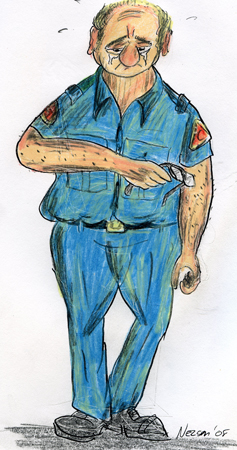
\includegraphics[height=60mm]{corps/chapitre15/img/personnage-timothee-pleur.jpg}
\end{floatingfigure}

L’improbable aveu a pour effet de pénétrer l’armature de Timothée qui, pour la deuxième fois de la journée, se retrouve entièrement déstabilisé et incapable de se contenir. Malgré une idée furtive indiquant qu’il torpillait toute chance, pour peu qu’il en eût, auprès de la belle infirmière, il se brise en sanglots.

- T’es bien chanceuse de le savoir, sanglote-t-il, moi, je ne l’ai jamais su. Va-t-y falloir que j’attende d’avoir 82 ans ?

Les mains sur la monture de ses verres, il part se réfugier dans la cuisine où, instantanément, Romain va l’enserrer dans ses bras. Gazou émet un début de grondement, mais il replace ses yeux sur Béatrice et reprend sa contemplation. C’est la vieille qui casse la glace, initiative qu’apprécie la visiteuse qui lutte elle-même pour ne pas chavirer dans les eaux de ses émotions.

- Ch’est vrai que je ne lui ai jamais dit que je l’aimais, pauvre p’tit garchon. Pourtant, pourtant …

Elle ne finit pas sa phrase.

- Maudite vie, reprend-elle. J’ai eu une vie complètement foquée.

Deuxième miracle de la soirée, Marie, fille de Marceline et d’Edmond Rioux, se met à se raconter, sans pudeur, sans le souci d’embarrasser cette étrangère qui semble si réceptive. Les mots vont sortir drus, puissants, libérés, comme une rivière longtemps empêtrée par un barrage de castor, ce qui lui a donné l’allure d’un petit lac, et qui, soudain, se met à couler et à couler. Pour la première fois de sa vie, la Maririou déballe son histoire. Elle se l’offre à elle, sans fixer personne, ni Romain ni Timothée qui se sont approchés, ni Béatrice dont les yeux sont humides. Elle regarde le tapis et, à grands coups d’archet, achève la destruction de sa maison de castor.

Au même moment sur la rue Crouet, une voiture est immobilisée en face du cimetière. Marie-Odile qui n’avait plus de Midol pour calmer ses douleurs était sortie s’en procurer à la pharmacie. À son retour, elle avait décidé de venir se «racheter» auprès de Timothée, convaincue que plus tôt dans la journée, elle n’avait pas été à la hauteur de l’accablement avec lequel il était aux prises. En débouchant sur la rue, elle a aperçu une voiture stationnée devant la maison de son amant, phénomène inhabituel puisqu’il déplorait ne jamais recevoir de visiteurs, et, en femme flic, bien que lourdement menstruée, elle a voulu savoir qui en était le propriétaire. Utilisant sa boucle d’oreille et certaines habiletés policières, elle a fait une courte recherche et a pu apprendre que la bagnole était au nom d’une certaine Béatrice Martin.

C’est ce véhicule qu’elle regarde présentement, la mâchoire crispée et les yeux en tempête.